\section{Introduction}
\label{sec:introduction}
% the problem we are solving, distinguish with previous problems
In the applications like street navigation~\cite{ohno2003outdoor}, visual-based 6-DOF camera pose estimation~\cite{campbell2017globally,moreno2008pose,Kendall_2015_ICCV,coskun2017long} providing high accuracy attracts much attention in computer vision.
Additionally, to acquire better scene understanding for semantics applications such as augment reality~\cite{DBLP:journals/corr/abs-1708-05006}, parsing each frame of a video is also important.

\begin{figure*}[t]
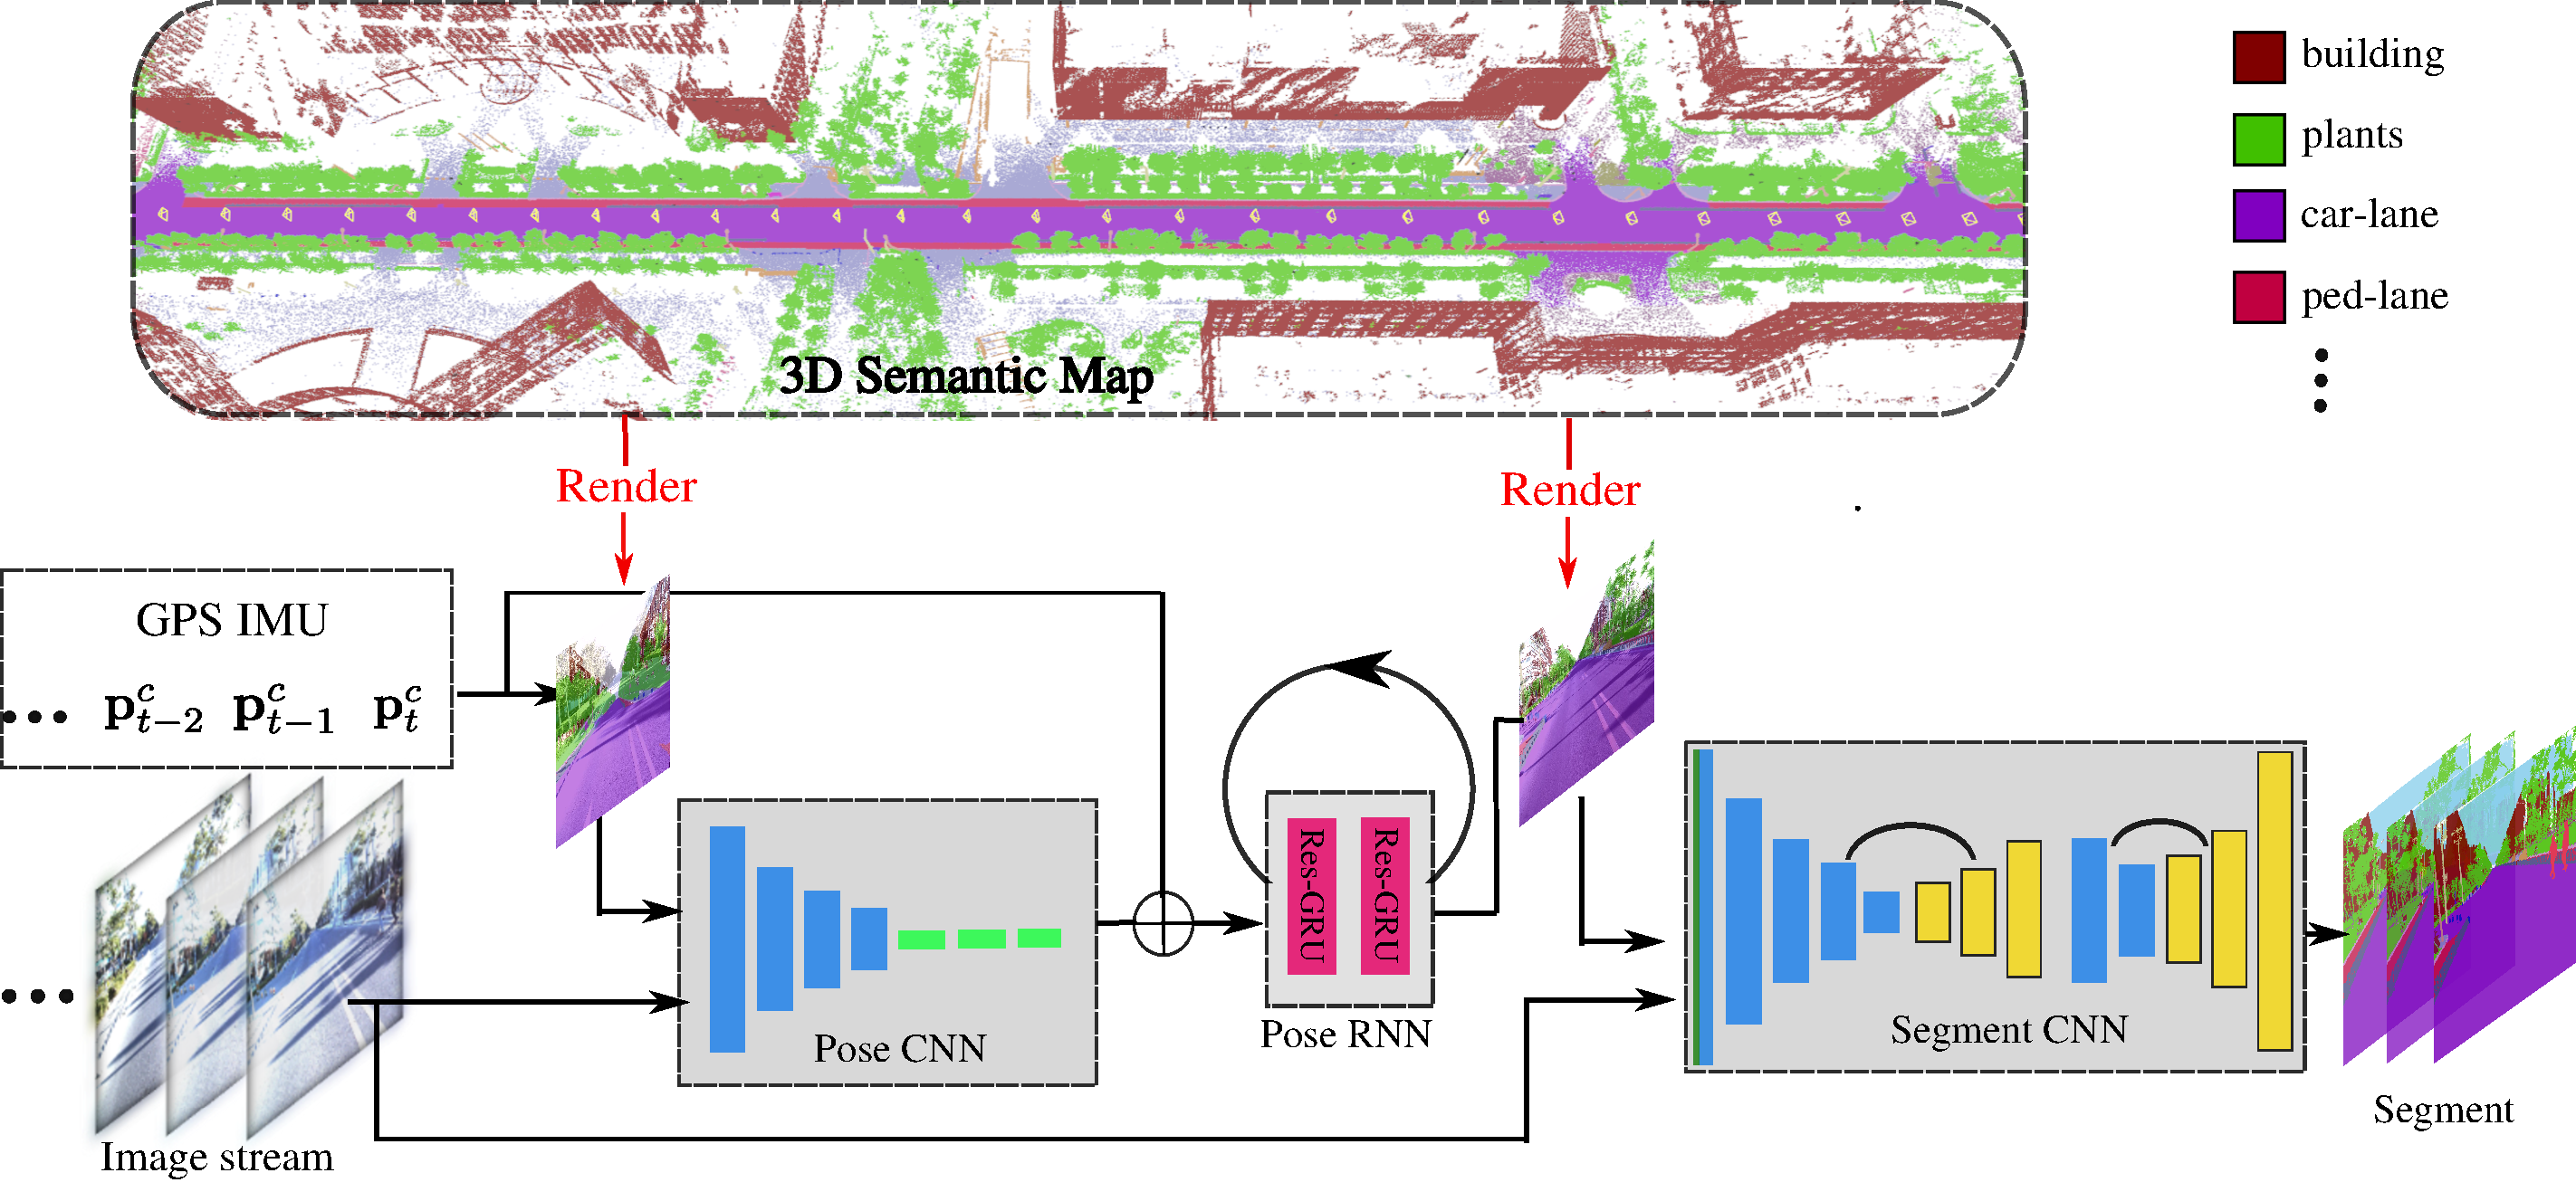
\includegraphics[width=\textwidth]{fig/framework.pdf}
\caption{Framework of our proposed system. The black arrows show the testing process, and red arrows show the render operation.}
\label{fig:framework}
\end{figure*}

% existing methods only consider one of the tasks with soly visual signal.
Currently, most existing vision algorithms are trying to solve both of the tasks solely depend on visual signals.
For instances, geometric based methods are relying on visual feature matching, \eg system of Perspective-n-Points (PnP)~\cite{haralick1994review,kneip2014upnp,campbell2017globally} when a 3D map and an image is provided, or systems of SLAM~\cite{engel2014lsd,mur2015orb,NewcombeLD11} when it is a video. Such systems are relying on local appearance, which could fail when confronted of low-texture environments.

Most recently, deep learning based methods, \eg either for images~\cite{Kendall_2015_ICCV} or videos~\cite{DBLP:journals/corr/ClarkWMTW17}, are proposed for real-time localization, which show much better trade-off between accuracy and speed.
Nevertheless, those monocular methods are good for environments with rich distinguishable features, \eg, Cambridge landmarks~\cite{Kendall_2015_ICCV}, while could fail for common street views with very similar appearances. For example, when driving forward with same trees beside, can hardly localize the images without external signals.

For scene parsing, approaches~\cite{ZhaoSQWJ16,ChenPSA17} based on deep fully convolutional network (FCN) with ResNet~\cite{HeZRS15} are the best algorithms for single image according to Dataset like CityScape~\cite{Cordts2016Cityscapes}. When input is videos, researchers~\cite{kundu2016feature,zhu2016deep} may incorporate optical flow between consecutive frames, which accelerates the parsing, and builds the consistency along the temporal dimension. Furthermore, for background, one may factorize the flow to 3D map and pose through structure-from-motion (SFM)~\cite{wu2011visualsfm}, so that jointly parsing and reconstruction~\cite{kundu2014joint} can performed. However, these methods are still not efficient enough and facing challenges of scene variations cross different weathers and cities for real applications.

In our scenario, targeting at a more practical setting, we consider the video is online recorded, and a 3D semantic map is pre-built by us. For handling the localization confusion of street views, we propose to fuse signals from motion sensors like global positioning system (GPS) and inertial measurement unit (IMU), which is typically available for current navigation system. Those signals can be noisy but is crucial as a pose priori for our deep learning system.
For video segmentation, we online render images from the 3D map, which serves as a priori for further segmentation, and helps the consistency along the temporal dimension.

%
In fact, our problem setting is on par with the widely applied mobile navigation system, whereas the 2D labeled map is raise up to a 3D semantic map, and the problem of 2D pose estimation is changed to 3D camera pose. Promisingly, lots of city scale 3D map has already collected from companies such as Google Earth~\cite{sheppard2009ethics} and Altizure\footnote{https://www.altizure.com/}, and also semantic labeled ones is also built such as Toronto city~\cite{wang2016torontocity}. In our case, we constructed our own data with high quality 3D semantic map, by adopting a high accurate LIDAR device called Riegl\footnote{http://www.rieglusa.com/index.html}.

Last but not the least, within our deep learning framework, the camera pose and semantics are mutually beneficial, where pose helps build the correlation between the 3D semantic map and 2D semantic segments. Reversely, semantics could help align camera poses, yielding better results for both tasks than doing them individually. In our experiments, using a single core of Titan Z GPU, our system estimates the pose in 10ms with accuracy under 1 degree, and segments the image $512 \times 608$ in less than 100ms with pixel accuracy around 96$\%$, which demonstrates its efficiency and effectiveness.

% redefine our problem
In summary, the contributions of this paper are in three folds:
\begin{itemize}
    \item We propose a deep learning based system for fusing multiple information, \ie camera, GPS and IMU, and 3D maps, which helps to improve the robustness and accuracy for camera localization and scene parsing.
    \item In our system, camera pose and scene semantics are handled jointly in both training and testing, where two kinds of information are mutually beneficial.
    \item To evaluate based on the setting of problem, we construct a dataset from real scenes. It includes dense 3D semantically labelled point cloud, ground truth camera poses and pixel-level parsing of every frame, which we will release in order to benefit the related research in computer vision.
\end{itemize}

The structure of this paper is organized as follows. We first give a overview of our system in \secref{sub:framework}. In \secref{sec:data_collection}, we first describe how our data is different from the existing outdoor datasets. In addition, we briefly introduce the method how the data is collect and labelled. Then, \secref{sec:localize_and_parsing} presents the framework and detail of our system. The full performance is evaluated quantitatively for both pose estimation and parsing in \secref{sec:experiments}, and \secref{sec:conclusion} concludes the paper and point out future directions. Finally, We will release all our code, models and dataset with the publication of this paper.


\subsection{Framework}
\label{sub:framework}
The framework of our system is illustrated in \figref{fig:framework}. At above, a pre-built 3D semantic map is prepared. During testing, an online stream of images and corresponding camera poses are fed in to the system. Firstly, for each frame, a semantic label map is rendered out based on the obtained coarse camera pose. Then it is fed to a pose network jointly with the respective image.  The network calculates their relative rotation and translation, and yields a corrected camera pose. To build the temporal correlations, the corrected poses are fed into a RNN which further improve the pose accuracy in the stream.
Last, given the rectified camera pose, a new rendered label map is generated. We feed it together with the image to a segmentation network, which helps to segment a spatially more accurate and temporally more consistent result for the stream of video.
In this system, since our data contains ground truth for both pose and segments, it can be trained with strong supervision at each end of outputs.
